
\begin{frame}{Ambient Light - Global Illumination Approximation}
  \begin{columns}
    \begin{column}{0.6\textwidth}
      \begin{raybox}{Ambient Light Purpose}
        \textbf{Problem:} Real scenes have indirect lighting
        \begin{itemize}
          \item Light bounces off walls, ceiling, floor
          \item Multiple reflections illuminate shadows
          \item Even "dark" areas receive some light
        \end{itemize}

        \vspace{0.3cm}
        \pause
        \textbf{Solution:} Add constant ambient term
        \begin{itemize}
          \item Prevents completely black shadows
          \item Approximates global illumination
          \item Simple and fast to compute
        \end{itemize}

        \vspace{0.3cm}
        \pause
        \textbf{Formula:}
        \begin{align}
          I_{\text{ambient}} = k_a \cdot I_a
        \end{align}
        where $k_a$ is ambient coefficient, $I_a$ is ambient intensity
      \end{raybox}
    \end{column}
    \begin{column}{0.4\textwidth}
      \begin{tikzpicture}[scale=0.8]
        % Room with indirect lighting
        \draw[thick] (0,0) -- (3,0) -- (3,3) -- (0,3) -- cycle;

        % Light source
        \node[circle, fill=LightColor, minimum size=0.6cm] (light) at (1.5,2.5) {};

        % Direct rays
        \draw[lightray] (light) -- (2.5,1.5);
        \draw[lightray] (light) -- (0.5,1.5);

        % Bounced rays (dashed)
        \draw[lightray, dashed, opacity=0.6] (2.5,0) -- (0.5,1);
        \draw[lightray, dashed, opacity=0.6] (3,1) -- (1,0.5);
        \draw[lightray, dashed, opacity=0.6] (0,2) -- (2,1);

        % Object in shadow
        \node[sphere, minimum size=0.6cm] (obj) at (1,1) {};

        % Labels
        \node[right] at (3.2,2) {\footnotesize Direct light};
        \node[right] at (3.2,1) {\footnotesize Bounced light};
        \node[below] at (1,0.4) {\footnotesize Still receives};
        \node[below] at (1,0.1) {\footnotesize some light};
      \end{tikzpicture}
    \end{column}
  \end{columns}
\end{frame}

\begin{frame}{Light Attenuation Models Summary}
  \begin{center}
    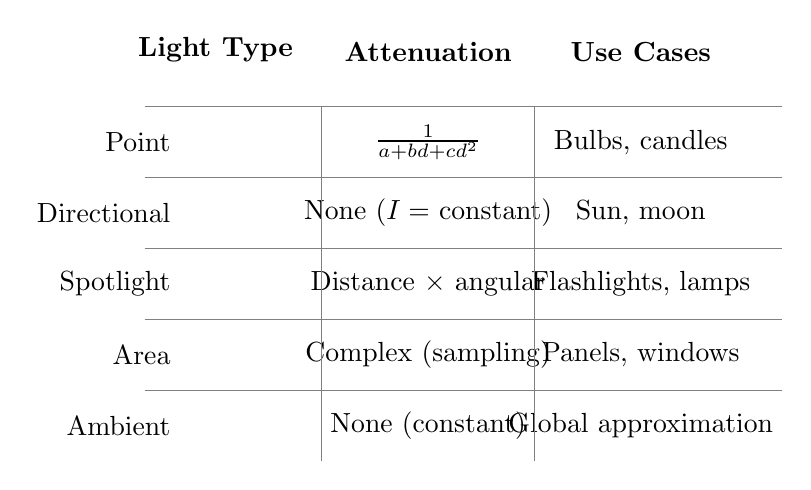
\begin{tikzpicture}[scale=0.9]
      % Comparison table
      \node[above] at (0,3) {\textbf{Light Type}};
      \node[above] at (3,3) {\textbf{Attenuation}};
      \node[above] at (6,3) {\textbf{Use Cases}};

      % Point light
      \node[left] at (-0.5,2) {Point};
      \node at (3,2) {$\frac{1}{a + bd + cd^2}$};
      \node at (6,2) {Bulbs, candles};

      % Directional light
      \node[left] at (-0.5,1) {Directional};
      \node at (3,1) {None ($I = $ constant)};
      \node at (6,1) {Sun, moon};

      % Spotlight
      \node[left] at (-0.5,0) {Spotlight};
      \node at (3,0) {Distance $\times$ angular};
      \node at (6,0) {Flashlights, lamps};

      % Area light
      \node[left] at (-0.5,-1) {Area};
      \node at (3,-1) {Complex (sampling)};
      \node at (6,-1) {Panels, windows};

      % Ambient
      \node[left] at (-0.5,-2) {Ambient};
      \node at (3,-2) {None (constant)};
      \node at (6,-2) {Global approximation};

      % Draw grid
      \foreach \y in {2.5,1.5,0.5,-0.5,-1.5} {
        \draw[gray] (-1,\y) -- (8,\y);
      }
      \foreach \x in {1.5,4.5} {
        \draw[gray] (\x,-2.5) -- (\x,2.5);
      }
    \end{tikzpicture}
  \end{center}

  \vspace{0.5cm}
  % IMAGE: Side-by-side comparison of all light types
  % Show same scene lit with different light types
  % \includegraphics[width=\linewidth]{images/light_types_comparison.jpg}
  \textcolor{gray}{[Comparison of all light types on same scene]}
\end{frame}